\documentclass[12pt]{article}

\usepackage{graphicx}
\usepackage[sorting=none]{biblatex}
\usepackage[margin=1in]{geometry}
\usepackage[colorlinks=true]{hyperref}
\usepackage{amsmath}
\usepackage{amssymb}
\usepackage[format=plain, labelfont=it, font=footnotesize, labelsep=period]{caption}
\usepackage{caption}
\usepackage{subcaption}

\addbibresource{references.bib}

\title{Pendulum Lab Report II}
\author{Kevin (Zerui) Wang}
\date{\today}

\begin{document}

\pagenumbering{gobble}

\maketitle
\newpage

\pagenumbering{arabic}

\section{Introduction}
{\color{blue}The purpose of this lab report is to evaluate the accuracy of various theoretical models used to predict the behaviour of a simple pendulum.}

The first part of this lab report focuses on the relationship the period and release angle of a simple pendulum. After results were collected and analyzed, an improved version of the pendulum was created to collect angular data in order to determine the Q factor.

{\color{blue}Lastly, further analysis was done on the Q factor to try to determine a trend in relation to the pendulum length}

\section{Background} \label{Background}
{\color{blue}A simple pendulum can be defined as a weight suspended below a pivot point to which it swings back and forth freely along a plane that contains the pivot point via a flexible string. The length of the pendulum is defined as the distance from the pivot to the center of mass of the weight hanging from the pendulum. Usually, the weight of the string is negligible in comparison to the pendulum mass.} For a simple pendulum of length $L$ experiencing a downwards force due to gravity $g$, the period $T$, for a release angle $\theta$, is given by the following equation \cite{the-simple-pendulum}:
\begin{equation} \label{eq:l-over-g}
    T = 2\pi \sqrt{\frac{L}{g}}
\end{equation}

{\color{blue}Note that Equation \ref{eq:l-over-g} does not depend on $\theta$ because it represents the behaviour of an ideal pendulum.} More realistically, the behavior of a pendulum assuming no energy loss due to friction can be modelled with a second order differential equation of $\theta$ with respect to $t$:
\begin{equation} \label{eq:diffeq-pendulum}
    \frac{d^2\theta}{dt^2} + \frac{g}{L}\sin{\theta} = 0
\end{equation}
{\color{blue}which cannot be solved in terms of elementary functions \cite{no-elementary-fns}. However, if small angle approximation is assumed, where $\sin\theta \approx \theta$, the differential equation can be rewritten and solved to yield $\theta(t)$ in terms of a sine wave with period of Equation \ref{eq:l-over-g}. For $|\theta| \lesssim 20^{\circ}$, small angle approximation (and therefore simple harmonic motion) holds \cite{the-simple-pendulum}.} Additionally, the the mass of the pendulum weight does not show up in any of the equations, implying that pendulum period does not depend on mass for the previous models.

Another way to model a pendulum realistically is to incorporate dampening from air resistance and friction within the string fibres, given by the following equation \cite{damped-oscillations}:
\begin{equation} \label{eq:damped-harmonic-oscillator}
    \theta(t) = \theta_0 e^{-{t/\tau}} \cos\left(2\pi\frac{t}{T} + \phi_0\right)
\end{equation}
where $\theta_0$ is the initial release angle in radians, $T$ is the pendulum's period, $\phi_0$ is the angular phase shift, and $\tau$ {\color{blue} is the decay constant that governs all factors that results in the damped harmonic motion. However, it can be inferred from this model that $T$ is constant, implying the presence of small angle approximation.}

{\color{blue}
Additionally, the amplitude-time graph of the pendulum can be modelled by removing the cosine term from Equation \ref{eq:damped-harmonic-oscillator}:
\begin{equation} \label{eq:amplitude-function}
    A(t) = \theta_0 e^{-{t/\tau}}
\end{equation}}

In order to quantify the dampening effect of a pendulum, its Q factor may be used. The Q factor measures how damped an oscillator is and is defined as follows. \cite{pnp-physics}:
\begin{equation} \label{eq:q-factor-formula}
    Q = \pi\frac{\tau}{T}
\end{equation}

The Q factor also represents the the number of oscillations for the pendulum's amplitude to decay to $e^{-\pi}$, or $\approx 4\%$ of its original amplitude. {\color{blue}However, it suffices to count $Q/n$ swings where the amplitude decays to $e^{-\pi/n}\,\%$ of its original. Qualitatively, when the Q factor is large, the pendulum comes to rest slower. When the Q factor is small, the pendulum comes to rest quicker.}

\newpage

\section{Period and Release Angle}

\subsection{Experimental Setup}
The initial setup for the pendulum was made by first attaching a protractor on a desk. The pendulum, made by tying a piece of cotton string around a stainless steel quick link {\color{blue} that was aligned to match the $90^{\circ}$ mark on the pendulum. Extra tape was also used to reinforce the pivot point, which was made to be collinear to the $0^{\circ}$ and $180^{\circ}$ markings.} The length of the pendulum was measured using measuring tape. An image of the experimental setup is shown below:

\begin{figure}[!hptb]
    \centering
    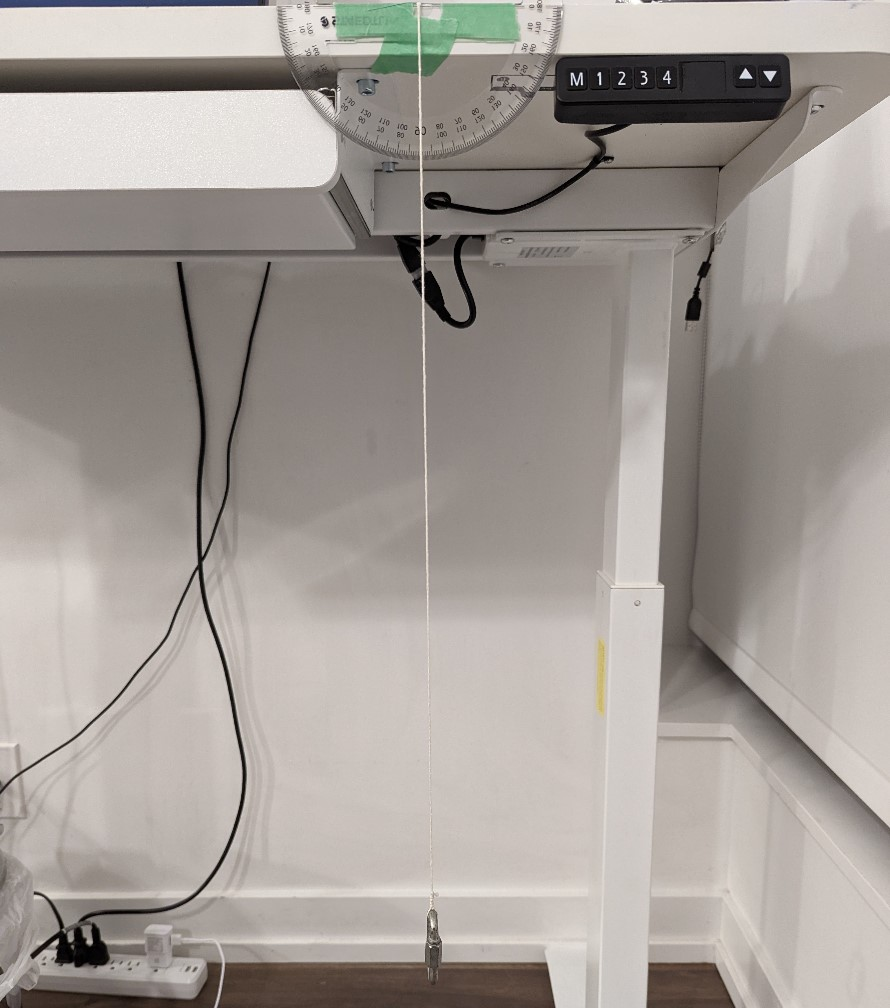
\includegraphics[width=0.5\textwidth]{../figures/exp_setup1.jpg}
    \caption{\centering Picture of experimental setup for period vs. release angle data collection}
    \label{fig:figure 1}
\end{figure}

\newpage

\subsection{Data}
The data collected for the period vs. release angle graph is shown in the plot below:

\begin{figure}[!hptb]
    \centering
    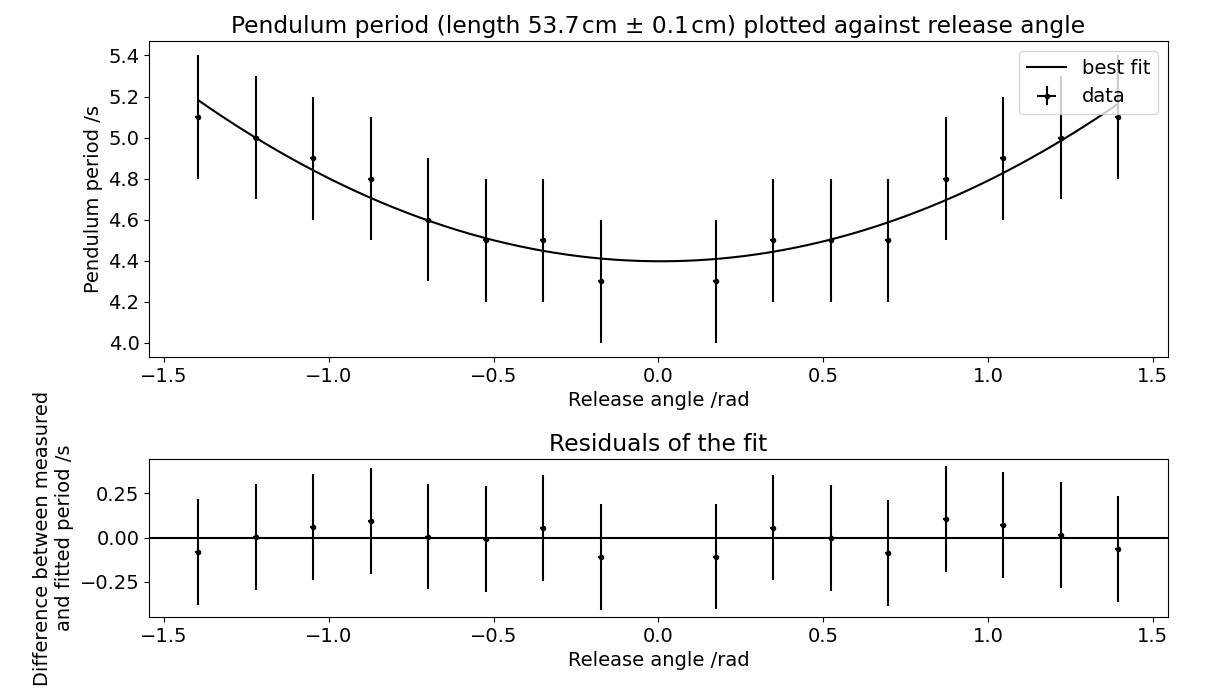
\includegraphics[width=\textwidth]{../figures/period_vs_release_angle.png}
    \caption{\centering Period plotted against release angle of the setup in Figure \ref{fig:figure 1}}
    \label{fig:figure 2}
\end{figure}

All data collected for this graph were done without the need for tracking software. {\color{blue}In total, 8 angles were recoded from both sides of the pendulum, starting from $10^\circ$ and taking increments of $10^\circ$ up to $80^\circ$}. The uncertainty for the protractor (measured by eye) was taken to be the smallest increment, $0.5^{\circ}$ converted to radians, and the period uncertainty was taken to be the average human reaction time, $0.25\,\text{s}$ \cite{reaction-time} {\color{blue} since it is greater than the uncertainty of a stopwatch. The period itself was measured by recording the pendulum for 3 swings and dividing the total time by 3. The maximum height was taken as the reference point because there would be less certainty in the pendulum's position (lower speed).}

\subsection{Analysis}
According to Section \ref{Background}, {\color{blue} if $|\theta| \lesssim 20^{\circ}$, then a line of best fit with slope 0 would be expected, which is observed to happen for the 4 closes points plotted from a release angle of $0^\circ$. However, as the release angle increases, the overall trend deviates from Equation \ref{eq:l-over-g} and takes on more of a parabolic shape which can be modelled by a quadratic power series, which corresponds to the best fit line from Figure \ref{fig:figure 1}:}
\begin{equation} \label{eq:power series}
    T_0(1 + B\theta_0 + C\theta_0^2)
\end{equation}
where $T_0$ represents the period, $\theta_0$ the release angle and $B$ and $C$ some arbitrary constants. {\color{blue}Since the $r^2$ value is relatively close to 1, the residuals are small, and the graph passes through all error bars, this fit would be a valid representation of the trend. Additionally, the uncertainty for $T_0 = 0.03$, $B = 0.005$ and $C = 0.007$, calculated through fitting the trendline with a Python program.

The terms $B$ and $C$ are also significant because they describe the symmetry of parabola and how much it deviates from the trend described in Equation \ref{eq:l-over-g}. If $B$ does not equal 0, the parabola will not be centered at $\theta = 0$. Since the experimentally determined value of B is smaller than its uncertainty, it suffices to say that $B = 0$, which implies symmetry in the graph. On the other hand, if $C = 0$, then the line of best fit will have slope 0. However, this was determined experimentally to not be the case.


Lastly, the residuals shown on the graph do not suggest much asymmetry regarding the pendulum as the negative release angles appear symmetrical when compared to positive release angles. However, a single-stringed pendulum tends to spin in an elliptical fashion when released, affecting accurate measurements.

This, it can be concluded that the pendulum period depends on amplitude.}

\newpage

\section{Finding the Q Factor} \label{Finding the Q Factor}

\subsection{Experimental Setup}
{\color{blue}
A single-stringed pendulum tends to spin in an elliptical fashion when released. Not only does this violate the way a pendulum was defined in Section \ref{Background}, elliptical orbits may also lead to inaccurate measurements. To correct for this,} a degree of freedom was removed from the pendulum by threading a string through the stainless steel quick link and fastening the 2 strings in 2 locations to form the shape of a ``V''. Then pendulum would then swing back and forth in the plane perpendicular to the ``V'', and the tendency for each string to balance out the load prevents it from swinging in any other direction. Additionally, the pendulum was kept the same length as the previous setup (perpendicular distance from threading location to top of desk), and extra precautions were taken to make sure the pendulum was symmetrical along the vertical axis. Below is a setup of what was described above:
\begin{figure}[!hptb]
    \centering
    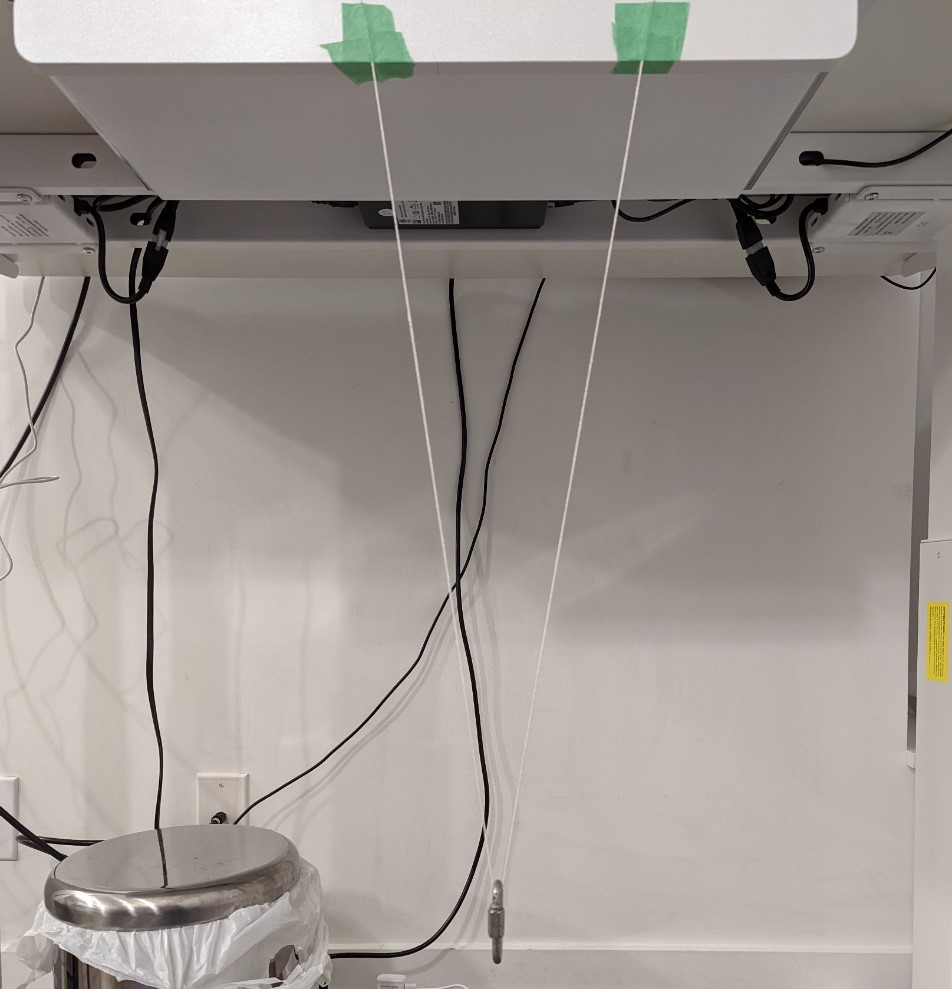
\includegraphics[width=0.5\textwidth]{../figures/exp_setup2.jpg}
    \caption{\centering Improved version of the pendulum used to determine Q factor}
    \label{fig:figure 3}
\end{figure}

\newpage

\subsection{Data}
{\color{blue}
is still referring to old lab data
- version 2 of the pendulum was released from a large angle, and it was deconstructed a long time ago, no access to it.
- version 3 of the pendulum (figure x) was used for
- mention uncertainty of angle due to tracker, and include an image
- the first version of this graph was generatred with an initial release angle of 60 degrees, but that doens't work, as shown earlier that the period depends on the release angle, which also implies that the period is not constant as the pendulum dampens, which creates a contradiction with Eq x.

- after observing results of lab 1,  the new and improved version is generated with a initial release angle of about 20 degrees, makes sure that the period stays constant, that was the theoretical model holds

- uncertainy now is 1/30 where 30 represents the frame rate of the videos.

- the length of the video was divided into around 15-20 equal intervals, and a few frames were advanced or retraced using tracker to determine the closes "peak"  - this is how I recorded the data

also mention the 20 second increments that were used because the full video was recorded (this was mentioned in section 6 or smth, move that here)



}
Due to the double-string contraption, the camera must be positioned in a place where the chance of capturing both strings in the same frame is minimized.

A protractor was not included in the experimental setup this time because Tracker \cite{tracker} was used to measure the angles. First, data was collected such that the maximum amplitude of the pendulum could be plotted against time:

\begin{figure}[!hptb]
    \centering
    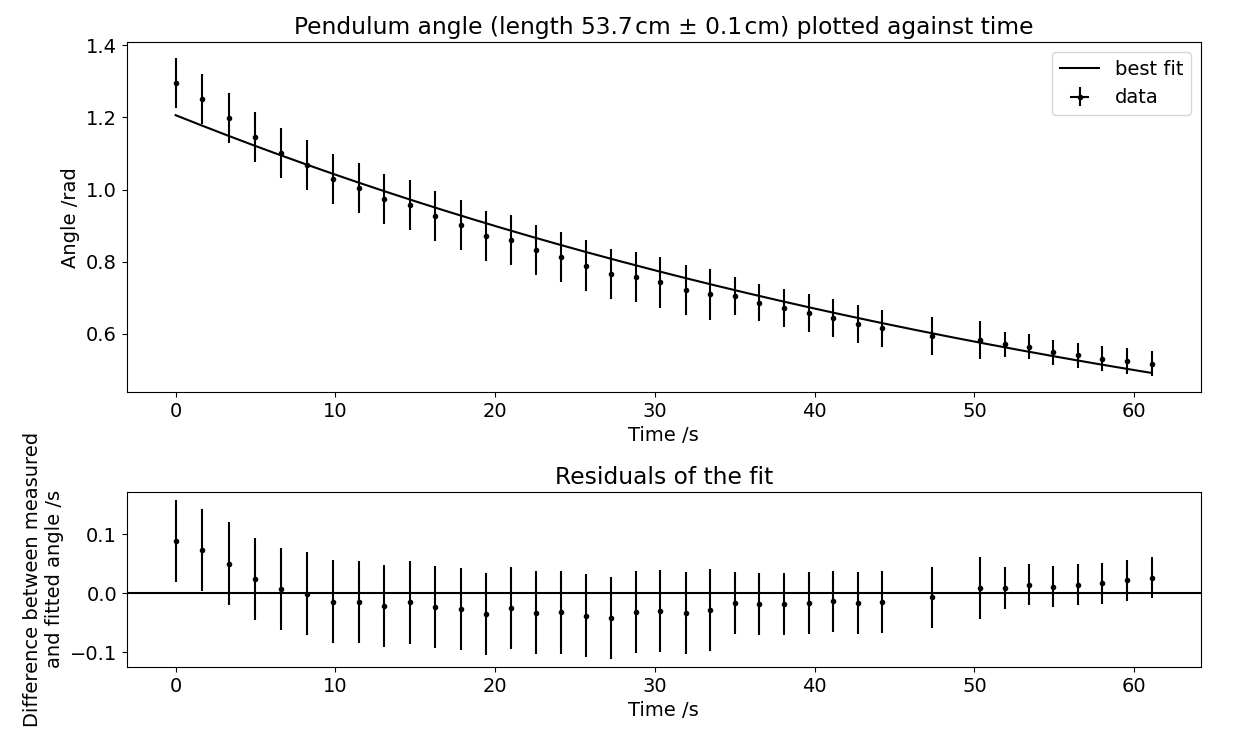
\includegraphics[width=\textwidth]{../figures/max_amplitude_vs_time.png}
    \caption{\centering Graph of maximum amplitude vs. time}
    \label{fig:figure 4}
\end{figure}

The uncertainty for time was taken to be $1/f$ where $f$ represents the frame rate of the video imported into Tracker, namely $120\,\text{fps}$. The uncertainty for angle was calculated this time for each individual maximum by taking half the range of the sweeping area that the string made in Tracker due to video blur.


\subsection{Analysis}

{\color{blue}

- remember that q factor should be calculated by counting

- alos mention that when the amplitude decays to some value, the actual new amplitude may not correspond to a peak, but some angle of pendulum swing in between the peak


- when the penulum decays to a certain amplitude that corresponds to some q/n, nez, it corresponds to a time in the graph

- due to the nature of the exponential decay function,

}


The exponential fit used to create a curve of best fit for the data was taken from Equation \ref{eq:damped-harmonic-oscillator}, removing the periodic motion portion. The equation for the fit is equal to:
\begin{equation}
    1.21e^{-{t}/68}
\end{equation}

With this information and also knowing the period ($1.67\,\text{s}$) of the pendulum when the release angle is $1.2064\,\text{rad}$, the $Q$ factor can be calculated. The uncertainty of the $Q$ factor is taken to be the largest percent uncertainty of $\tau$ and $T$.

$\tau$ was calculated to have an uncertainty of 1, which is less than the percent uncertainty of $T$, taken to be $0.3/1.67 \approx 15\%$. Thus, the value of $Q$ can be calculated to be $130 \pm 20$.

However, Graph \ref{fig:figure 4} can also be used to find the Q factor by counting the number of oscillations. Since the total amplitude does not decrease down to $e^-\pi \%$ of the original amplitude, it suffices to calculate a value for $Q/5$. The closes data points above and below $\theta_0e^{-{pi/5}}$ correspond to the $24^\text{th}$ and $25^\text{th}$ swing. Multiplying these values by 5 and taking half the difference (range) to be the uncertainty gives another Q factor of $123 \pm 2$.

%%%%%%%%%%%%%%%%%%%%%%%%%%%
%%%%%%%%%%%%%%%%%%%%%%%%%%%
%%%%%%%%%%%%%%%%%%%%%%%%%%%
%%%%%%%%%%%%%%%%%%%%%%%%%%%
%%%%%%%%%%%%%%%%%%%%%%%%%%%
% THIS IS ALL NEW
%%%%%%%%%%%%%%%%%%%%%%%%%%%
%%%%%%%%%%%%%%%%%%%%%%%%%%%
%%%%%%%%%%%%%%%%%%%%%%%%%%%
%%%%%%%%%%%%%%%%%%%%%%%%%%%
%%%%%%%%%%%%%%%%%%%%%%%%%%%

{\color{blue}

\section{Period and Length} \label{Period and Length}

\subsection{Experimental Setup}
A third version of the pendulum was made to collect data for 9 different lengths ranging from around $10\,$cm to $50\,$cm, as shown below:

\begin{figure}[!hptb]
    \centering
    \begin{subfigure}{0.49\textwidth}
        \centering
        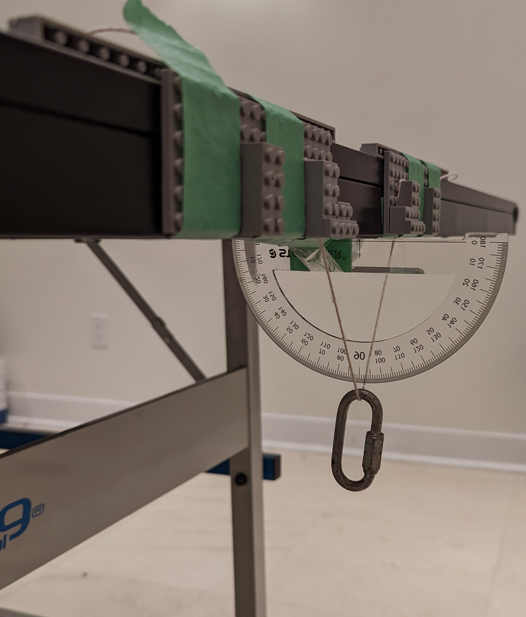
\includegraphics[width=\textwidth]{../figures/exp_setup3_angle.png}
    \end{subfigure}
    \hfill
    \begin{subfigure}{0.49\textwidth}
        \centering
        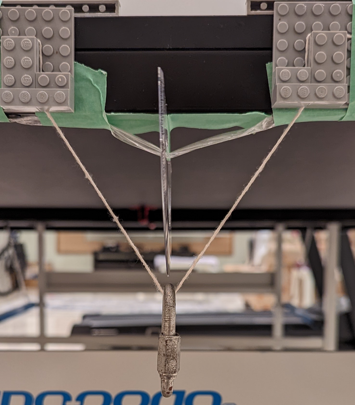
\includegraphics[width=\textwidth]{../figures/exp_setup3_front.png}
    \end{subfigure}
    \caption{Side and front view of version 3 of the pendulum}
    \label{fig:figure 5}
\end{figure}

The setup used here doesn't deviate much from the one used in Section \ref{Finding the Q Factor}, other than the fact that a real protractor was used in place of Tracker's virtual one, lego was used to prevent the potential risk of the string slipping under the tape and the angle formed by the ``V'' shape was kept to be around $60^\circ$ for all lengths recorded. The last point is especially important so that any dependent variable under investigation can only depend on one independent variable, the length of the pendulum.

Lastly, all angles were released from approximately $20^\circ$ to satisfy small angle approximation.

\subsection{Data}
Plotting period against length reveals a trend that looks like a square root function. Theoretically, this should be the case as shown by Equation \ref{eq:l-over-g}:

\begin{figure}[!hptb]
    \centering
    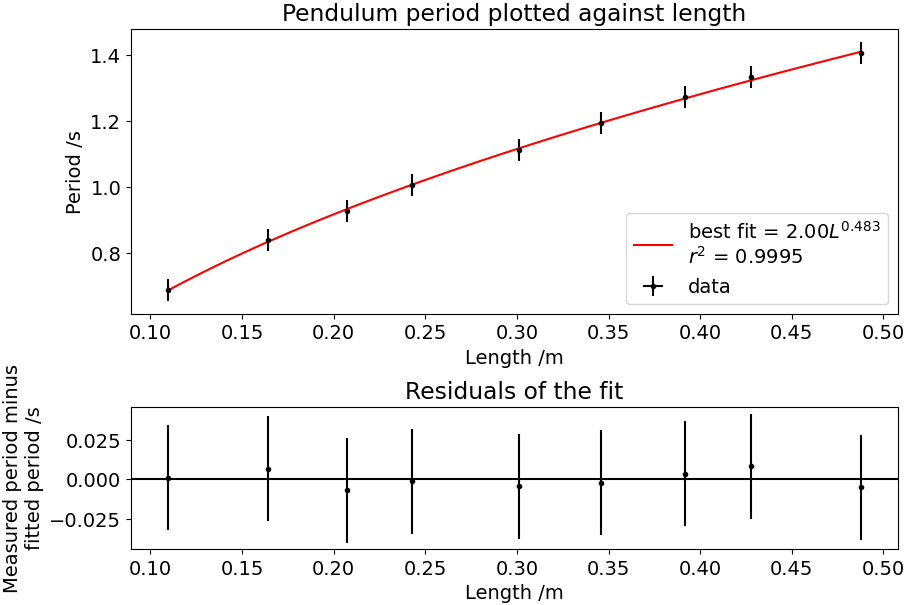
\includegraphics[width=\textwidth]{../figures/period_vs_length.png}
    \caption{Graph of pendulum period plotted against pendulum length}
    \label{fig:figure 6}
\end{figure}

a linear log-log plot of figure x can be shown to reinforce the idea that Equation x holds. I.e.

given the equation x, taking log on both sides results in <> and then the slope of the linear plot would be equal to n

The uncertainty for length was taken to be half of the smallest increment of a tape measure, multiplied by 2 since a double ended measurement was used. The uncertainty for period was taken to be 1/30, or how long a frame lasts

- talk about how I calculated uncertainty for the frame -> instead of using reaction time, I can loop the video by frames, as if it is frozen and then the uncertainty would decrease. the number of frames was recorded for 5 peak to peaks, and then converted into time and divided by 5


\subsection{Analysis}
Equation \ref{eq:l-over-g} can also be represented in the form of
\begin{equation}
    T = AL^{n}
\end{equation}
where $A = 2\pi/\sqrt{g}$ and $n = 0.5$.

From Figure \ref{fig:figure 6}, the uncertainty of $A = 0.01$ and $n = 0.004$, meaning that the experimentally determined value of A fits within the range of $2\pi/\sqrt{g}$ but B. However, the $r^2$ value for this fit, combined with low residuals implies that for small angles, the relationship between period and length is governed by Equation \ref{eq:l-over-g}.

\section{Q Factor and Length}

\subsection{Data}
The same setup from Section \ref{Period and Length} was used to calculate the Q factors. Videos of the pendulum almost swinging to rest were recorded for all lengths to more better capture the complete dampening of the pendulum.

The following graph was generated for the Q factor:
\begin{figure}[!hptb]
    \centering
    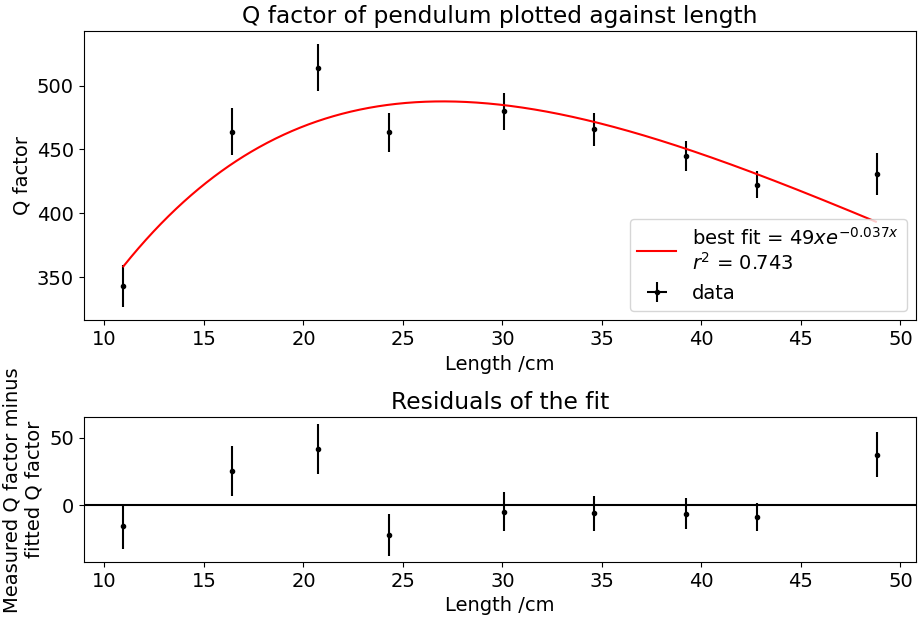
\includegraphics[width=\textwidth]{../figures/qfactor_vs_length.png}
    \caption{Graph of Q factor plotted against pendulum length}
    \label{fig:figure 7}
\end{figure}

- the uncertianty for q factor is inaccurate when measured with the counting method, which is outlines in an explnation in section <>


\subsection{Analysis}

- realizing the q factor peaks at a certain point
- air friction dominates after peak
- as the pendulum length gets longer, given the same release angle, the more gravitational potential energy it will have, which also implies the more velocity that it will hvae, and for fast speeds, velocity is porportional to v2, whereas for small velocities, velocity is porportional to v
- string friction dominates before peak
- additionally, the weight of the string may also be taken into account
- also the string has a surface area as well, which contributes to the drag force

- none of the fits seems to match with the trend of the graph
- fitting a cubic over this section does not make sense
- however, the graph looks like it follows the behaviour of a critically damped system.
- reference the equation of a critically damped system
- the critically damped system was modified to pass thorugh the origin because it would make sense for the q factor to equal to zero when when the lengh of the string equals 0 as well
- also the q factor shold approach 0 as the lenght of the string gets longer because there is more aerodynamic force. The graph should not cross the x axis because a negative q factor does not make sense

\section{Conclusion}
simple pendulum equation holds fo small angles

amplitude time graph also holds for small angles

the small angles stuff can be concluded based on the period vs release angle graph

q factor graph nobody knows what it is, I came up with a plausible function based off of intuition

}

\newpage

\printbibliography

\end{document}
